\section{Viabilidade Técnica}
\label{recursosHumanos}
\subsection{Metodologia}

A fase inicial do projeto, também conhecida como Ponto de Controle 1 (PC1), visa garantir a definição da Metodologia, da gestão de riscos, e as definições que farão parte do desenvolvimento. Nesse projeto, 
o objetivo principal na definição da metodologia e da cultura é garantir o desenvolvimento e a organização da condução do projeto e das atividades de acordo com praticas da comunidade Ágil e do  \textit{DevOps} já adotadas pela comunidade \cite{licorish2016adoption}. 

As práticas do  \textit{DevOps} farão parte dos objetivos principais do PC1, pois irão auxiliar na gestão do projeto, baseando-se em quatro categorias: \textit{People, Process, Delivery e Runtime} \cite{leite2019survey}. Desde o primeiro momento, foram aplicados e apresentados conceitos e práticas do  \textit{DevOps},  \textit{Lean} e Ágil. Essas práticas irão auxiliar na adoção de uma nova cultura ágil e colaborativa entre os membros do projeto para garantir a qualidade nos produtos desenvolvidos. 

Além dos conceitos técnicos e não técnicos do  \textit{DevOps}, foi adotado como base o \textit{framework Scrum}, em que empregamos processos e técnicas aos papéis, eventos, artefatos e regras, adaptando as necessidades da equipe. O objetivo do \textit{Scrum} no projeto é permitir o controle do trabalho a ser realizado por meio de uma gestão dinâmica, assim identificar obstáculos durante o processo de desenvolvimento, e reagir a eles se torna mais fácil \cite{gren2015prospects} \cite{gren2020agile} \cite{licorish2016adoption}. A abordagem interativa e incremental empregada otimiza a previsão e monitoramento de riscos.

Também adotamos o uso do  \textit{Kanban} para controle do fluxo de produção da equipe. Para a otimização do trabalho desta, foi utilizada a ferramenta  \textit{Trello}, já integrada no  \textit{MsTeams}. 

Para rastrear as tarefas e levantar dados, utilizamos o  \textit{Dashio} para coleta de Métricas e Indicadores que auxiliem as equipes. As Imagens \ref{fig:cumulativesoftware}, \ref{fig:cumulativeeletronica} e \ref{fig:cumulativeestrutura} apresentam o Gráfico \textit{Cumulative Flow} desse PC1 (Sprint 0 até 3). Pelo gráfico, podemos observar as entregas feitas a cada \textit{Sprint} (avanço no gráfico a cada 7 dias). O objetivo do time é reduzir o tempo entre as entregas para que não seja em formato de "pacotes" ao fim de cada revisão, garantindo assim uma entrega contínua. É possível observar que todos os times conseguiram fazer entregas durante a  \textit{sprint} e que na Imagem \ref{fig:cumulativesoftware} e \ref{fig:cumulativeeletronica} existem algumas distorções nos gráficos, pois os times identificaram duplicidade de atividades e arquivaram os \textit{Cards}.

\begin{figure}[H]
    \centering
  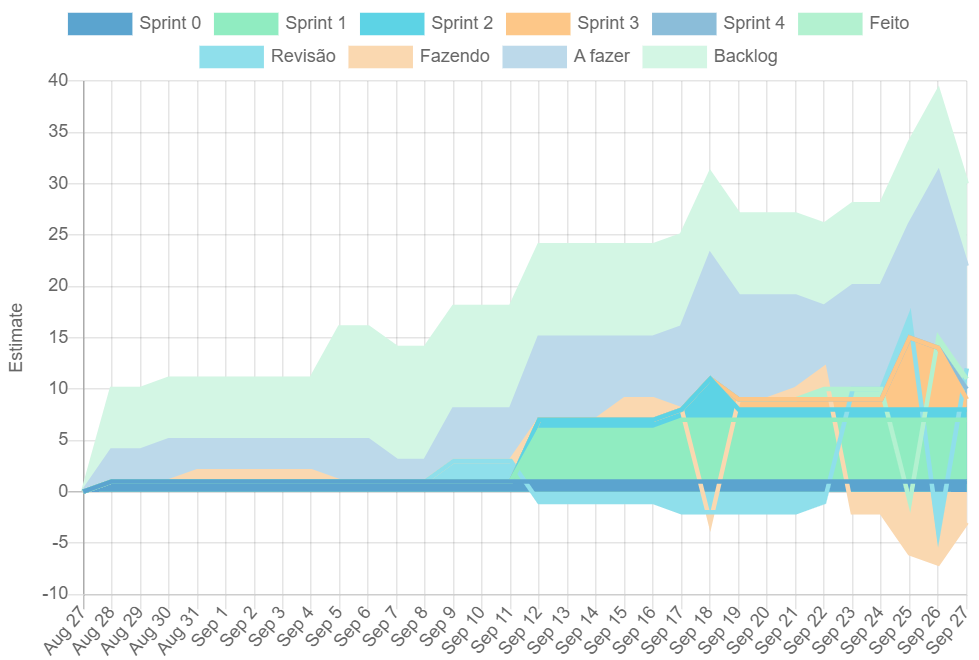
\includegraphics[scale=0.3]{figuras/cumulative_software.png}
  \caption{\textit{Cumulative Flow} da equipe de Software coletados de 27 de agosto até 26 de setembro de 2020.}
  \label{fig:cumulativesoftware}
\end{figure}
\begin{figure}[ht]
\centering
  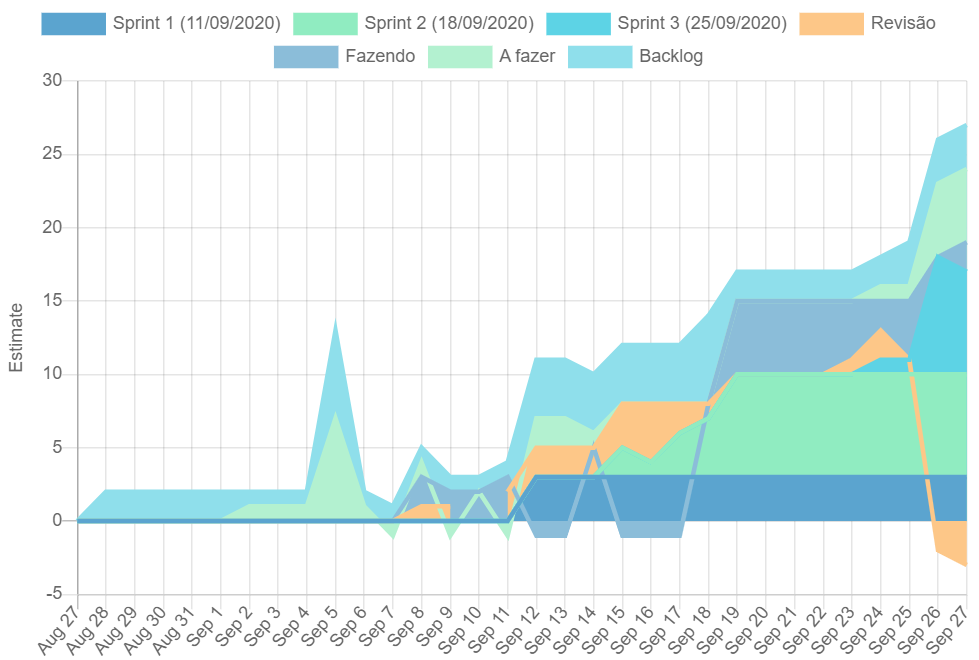
\includegraphics[scale=0.3]{figuras/cumulative_eletronica.png}
  \caption{\textit{Cumulative Flow} da equipe de Eletrônica coletados de 27 de agosto até 26 de setembro de 2020.}
  \label{fig:cumulativeeletronica}
\end{figure}
\begin{figure}[H]
\centering
  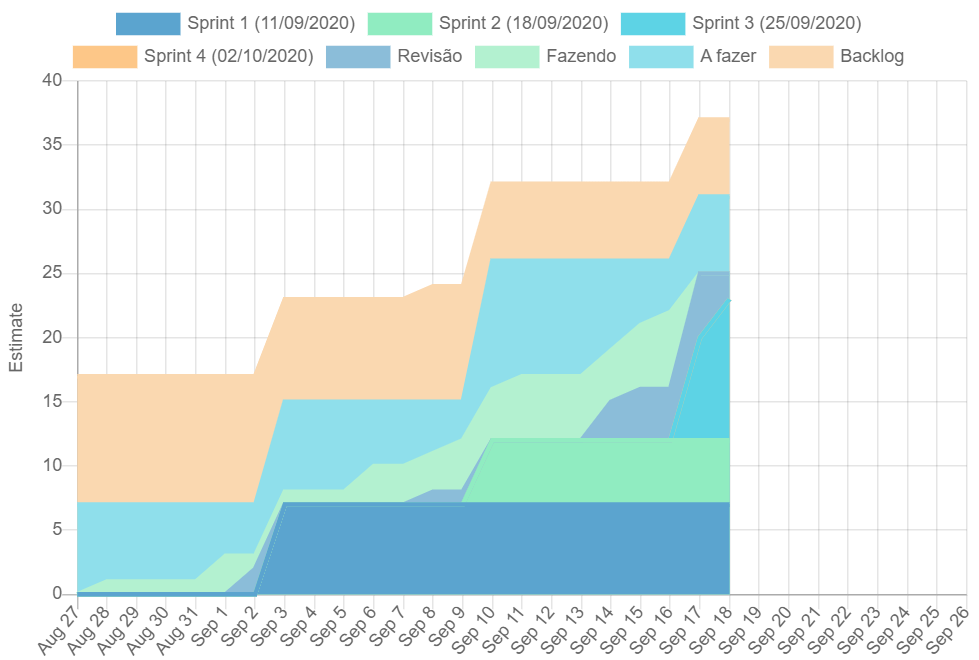
\includegraphics[scale=0.3]{figuras/cumulative_estrutura.png}
  \caption{\textit{Cumulative Flow} da equipe de Estrutura e Energia coletados de 27 de agosto até 26 de setembro de 2020.}
  \label{fig:cumulativeestrutura}
\end{figure}

Já o XP foi uma das metodologias adotadas pelo conjunto de práticas que são ditas como boas na Engenharia de Software como pareamento, refatorar o tempo todo, testar o tempo todo, entre outros.

\subsection{Papeis}
Durante o projeto, a equipe possuirá um Gerente Geral, um Diretor de Qualidade e será subdividida em 3 subgrupos, cada um contando com um Diretor Técnico (destacado em negrito):
\begin{itemize}
    \item Gerente Geral: Isaque Alves de Lima
    \item Diretor de Qualidade: Diogo Filipe Sens
    \item Estrutura e Energia
        \subitem - \textbf{Luisa Prospero de Carvalho Silva}
        \subitem - Artur Cardoso de Almeida
        \subitem - Douglas Alves Brandão 
        \subitem - Milena Martins Magalhães
        \subitem - Thainá Rodrigues Fernandes
    \item Eletrônica
        \subitem - \textbf{Gustavo Cavalcante Linhares}
        \subitem - Francisco Matheus Fernandes Gomes 
        \subitem - Misael de Souza Andrade
    \item Software
        \subitem - \textbf{João Henrique Egewarth}  
        \subitem - Andre Hernandez Bargas
        \subitem - Augusto Moreno Vilarins
        \subitem - Gabriela Alves da Gama
\end{itemize}

\subsection{Ritos Adotados}
\label{ritos}
\begin{itemize}
    \item \textit{Sprint}
        \subitem Início: sexta-feira
        \subitem Fim: sexta-feira
        \subitem Duração: 7 dias
\end{itemize}

\subsubsection{Planejamento da \textit{Sprint}}

\textbf{Duração máxima: 45 min}

A reunião de planejamento da  \textit{Sprint} é realizada semanalmente às sextas-feiras com a participação de todos os participantes separados nas suas frentes. A reunião de planejamento segue os seguintes passos:


1 - O time discute quais são as prioridades e necessidades do time;

2 - O time deve ter um objetivo bem definido para a  \textit{sprint};

3 - O time cria e seleciona as atividades que devem ser produzidas durante a  \textit{sprint};

\textbf{OBS:} Como as  \textit{sprints} são semanais, as atividades devem ser pensadas para concluir em 7 dias.

4 - Caso haja, o time deve definir e apresentar o pareamento da semana;

\textbf{OBS:} Esse pareamento deverá estar no definido na  \textit{issue}.

5 - Criar os  \textit{cards} no  \textit{Trello};

Deve conter nas  \textit{issues}:

- Titulo;

- Breve descrição;

- Responsável (no mínimo um);


\begin{itemize}
    \item\textbf{Entradas}
        \subitem \textit{Backlog} do produto;
        \subitem Último Incremento do produto;
        \subitem Desempenho na última \textit{Sprint}.
    
    \item\textbf{Saída}
        \subitem \textit{Backlog} da \textit{Sprint}.
\end{itemize}   


\subsubsection{Revisão da \textit{Sprint}}
\textbf{Duração máxima: 45 min}

\textbf{Missão:} Inspecionar o incremento e adaptar o \textit{Backlog}.

A reunião de Revisão do time é realizada semanalmente às sextas-feiras com a participação de todos os membros do time. A reunião segue os seguintes passos:

1 - O time discute e valida as atividades e artefatos produzidos durante a  \textit{sprint} que se finaliza;

2 - O time discute o \textit{Backlog} do Produto atual e se o time conseguirá atingir a meta das entregas;

3 - O grupo colabora com as soluções;

4 - É feita uma análise do mercado para definir o que é mais importante para fazer a seguir.


\subsubsection{Retrospectiva da \textit{Sprint}}
\textbf{Duração máxima: 30 min}


1 - Revisar, dentro do modelo de trabalho e das práticas do processo do  \textit{Scrum}, o processo de desenvolvimento, de forma a torná-lo mais eficaz e gratificante para a próxima \textit{Sprint};

2 - Inspecionar como correu a última \textit{Sprint} em se tratando de pessoas, das relações entre elas, dos processos e das ferramentas;

3 - Priorizar os principais itens que correram bem e aqueles que, se feitos de modo diferente, poderiam ter deixado as coisas ainda melhores.


\subsection{Ferramentas}
\begin{itemize}
    \item Teams
        \subitem Principal ferramenta de comunicação que permite o compartilhamento de vídeos, documentos e a integração com as outras ferramentas utilizadas no projeto, além de centralizar a comunicação ela é a ferramenta principal para as conferências.
    \item Drive
        \subsubitem Ferramenta em nuvem para armazenamento compartilhado. Será utilizada para compartilhar a documentação e informações entre os membros.
    \item Overleaf
        \subsubitem É uma ferramenta colaborativa de escrita online em LaTeX, cujo objetivo é facilitar todo o processo de escrita, edição e publicação de documentos.
    \item GitHub
        \subsubitem O GitHub é uma plataforma de hospedagem de código-fonte com controle de versão usando o Git.
\end{itemize} 